%!TEX TS-program = xelatex
\documentclass[]{friggeri-cv}
\usepackage{afterpage}
\usepackage{hyperref}
\usepackage{color}
\usepackage{xcolor}
\usepackage{smartdiagram}
\usepackage{fontspec}
% if you want to add fontawesome package
% you need to compile the tex file with LuaLaTeX
% References:
%   http://texdoc.net/texmf-dist/doc/latex/fontawesome/fontawesome.pdf
%   https://www.ctan.org/tex-archive/fonts/fontawesome?lang=en
\usepackage{fontawesome}
\usepackage{metalogo}
\usepackage{dtklogos}
\usepackage[utf8]{inputenc}
\usepackage{tikz}
\usetikzlibrary{mindmap,shadows}
\hypersetup{
    pdftitle={},
    pdfauthor={},
    pdfsubject={},
    pdfkeywords={},
    colorlinks=false,           % no lik border color
    allbordercolors=white       % white border color for all
}
\smartdiagramset{
    bubble center node font = \footnotesize,
    bubble node font = \footnotesize,
    % specifies the minimum size of the bubble center node
    bubble center node size = 0.5cm,
    %  specifies the minimum size of the bubbles
    bubble node size = 0.5cm,
    % specifies which is the distance among the bubble center node and the other bubbles
    distance center/other bubbles = 0.3cm,
    % sets the distance from the text to the border of the bubble center node
    distance text center bubble = 0.5cm,
    % set center bubble color
    bubble center node color = pblue,
    % define the list of colors usable in the diagram
    set color list = {lightgray, materialcyan, orange, green, materialorange, materialteal, materialamber, materialindigo, materialgreen, materiallime},
    % sets the opacity at which the bubbles are shown
    bubble fill opacity = 0.6,
    % sets the opacity at which the bubble text is shown
    bubble text opacity = 0.5,
}

\addbibresource{bibliography.bib}
\RequirePackage{xcolor}
\definecolor{pblue}{HTML}{0395DE}

\begin{document}
\header{Huynh Duc }{Dung}
      {Senior Full Stack Developer | AI Enthusiast}

% In the aside, each new line forces a line break
\begin{aside}
  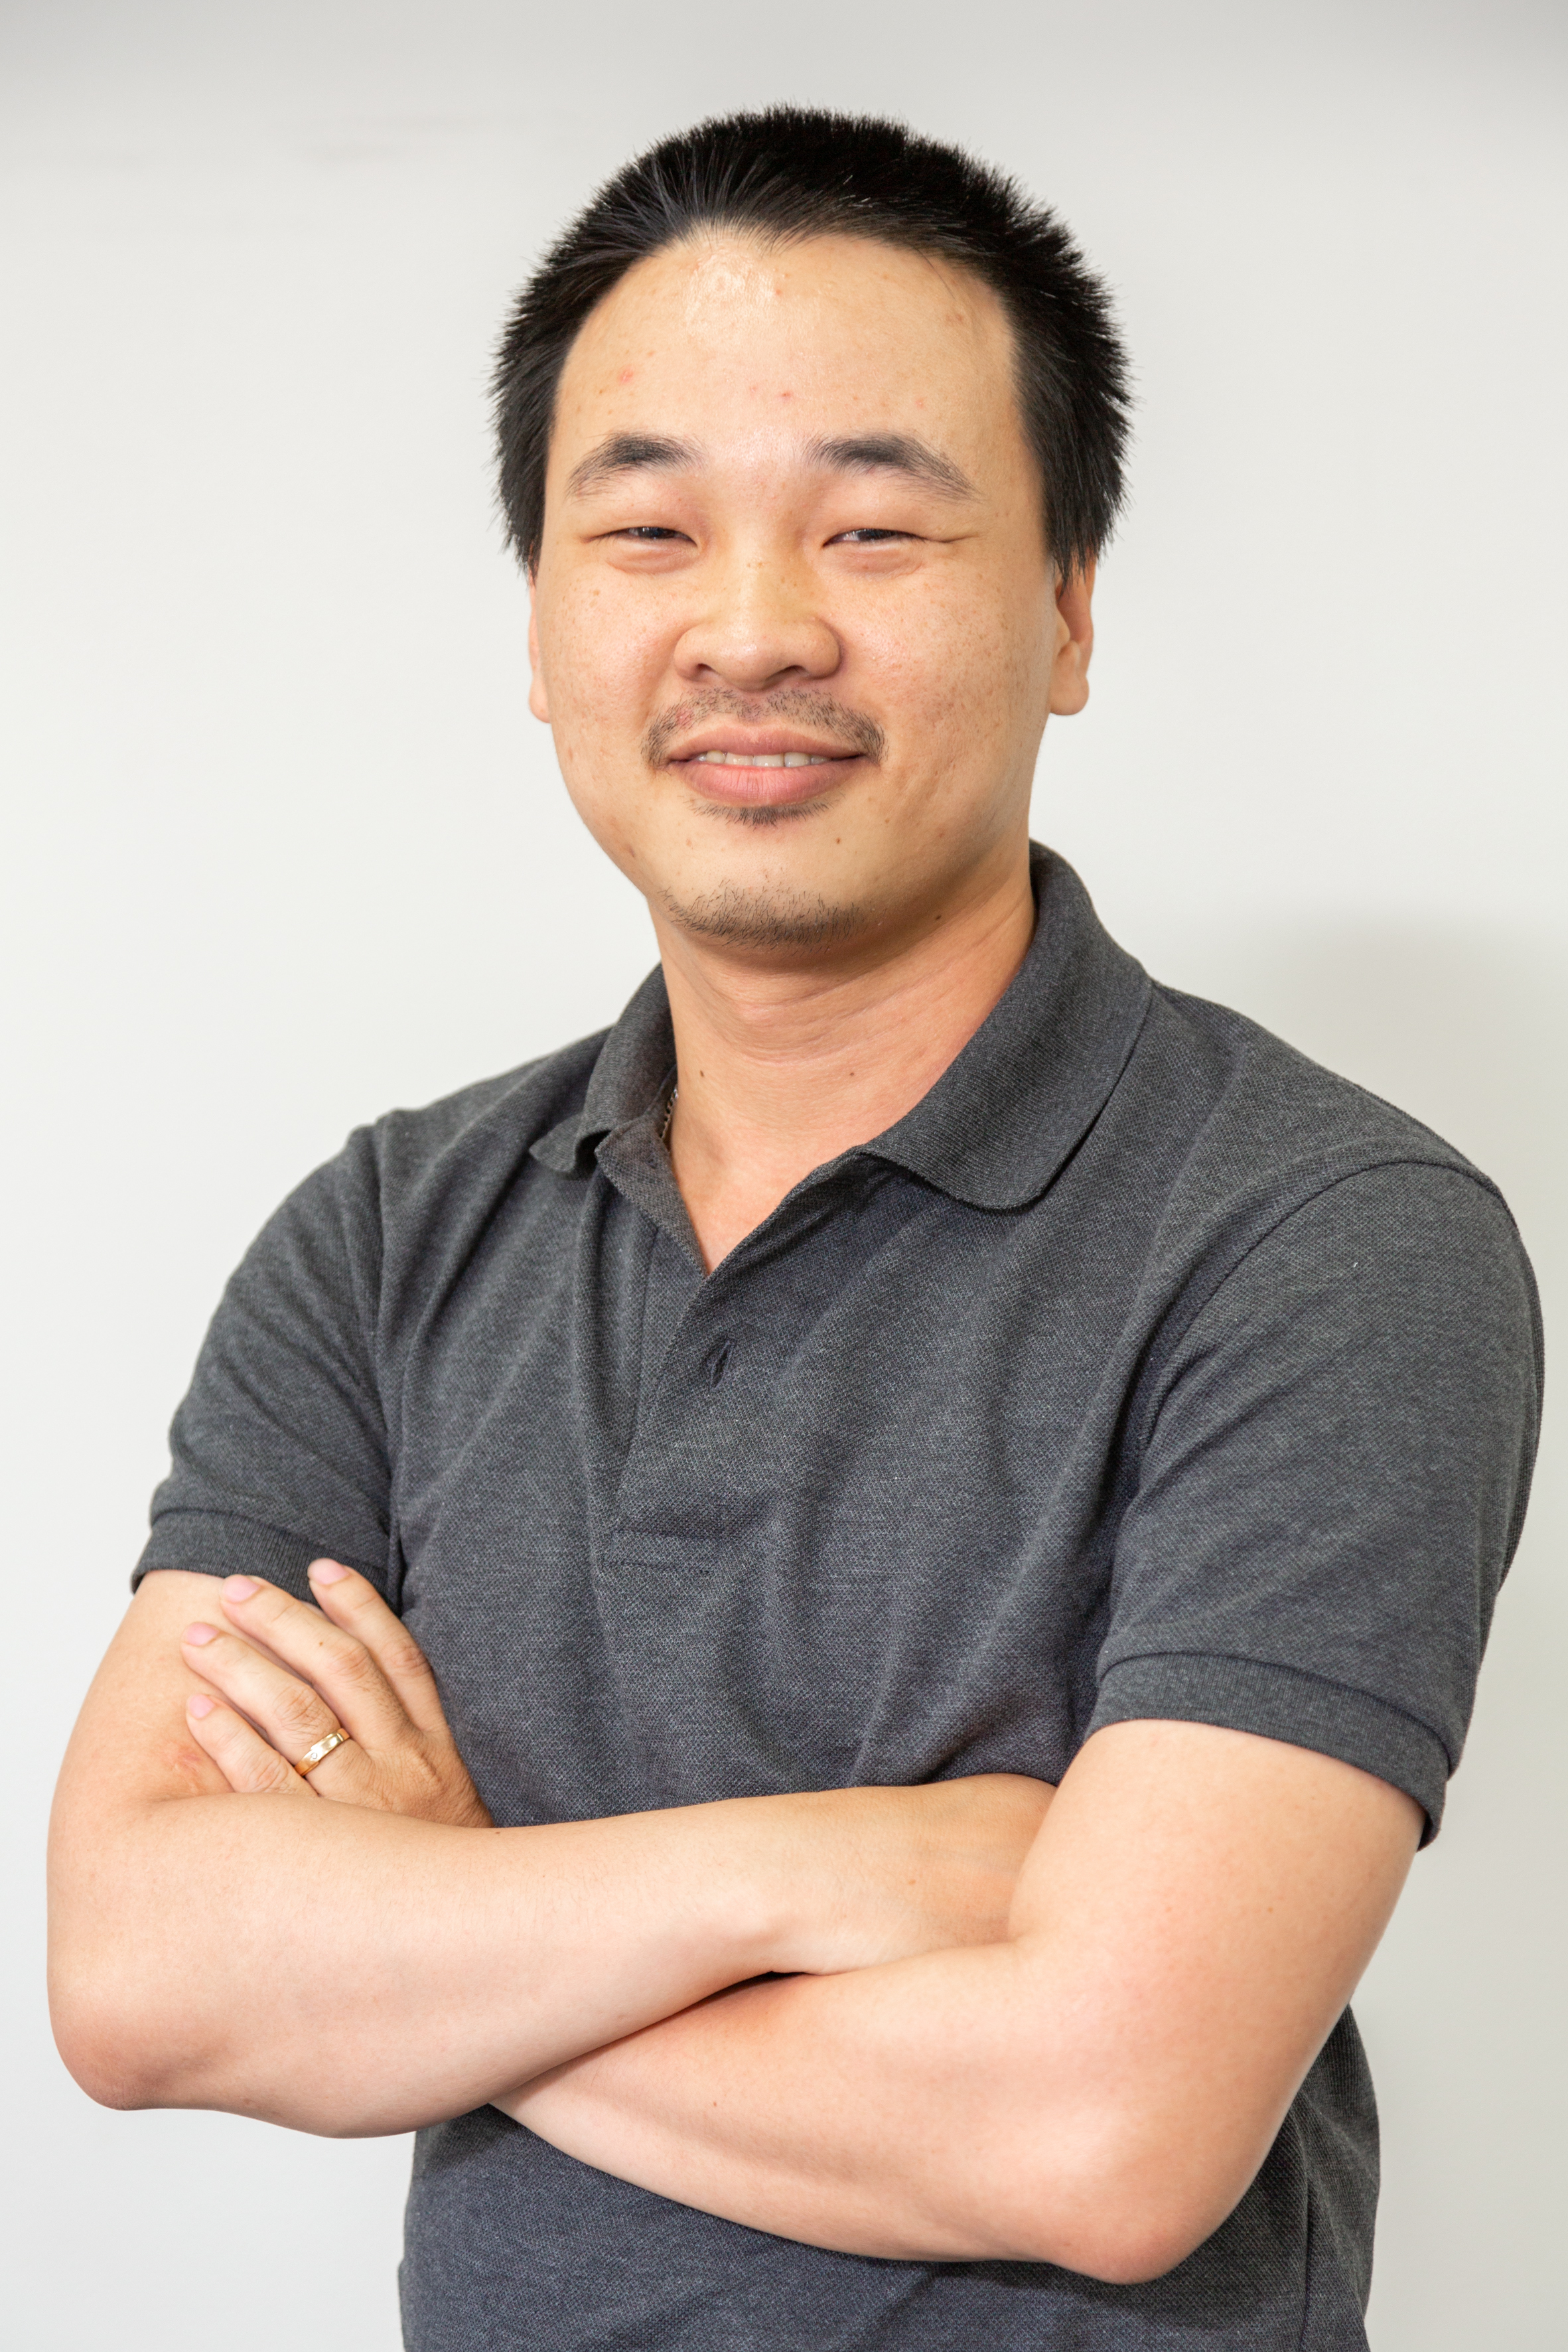
\includegraphics[scale=0.15]{img/Image-50.jpg}
  \section{Address}
   126 Lorong 1 Toa Payoh \#02-555 Singapore 310126
 \section{Nationality}
    Vietnam
    ~
  \section{Tel \& Skype}
    +65 89219468
    dunghd.it
    ~
  \section{Mail}
    \href{mailto:dunghd.it@gmail.com}{\textbf{dunghd.it@}gmail.com}
    ~
  \section{Web \& Git}
    \href{https://github.com/jellydn}{github.com/jellydn}
    \href{https://itman.fyi}{itman.fyi}
    \href{https://productsway.com}{productsway.com}
    \href{https://www.linkedin.com/in/dung-huynh-duc}{linkedin.com/in/dung-huynh-duc}
    ~
  \section{YouTube}
    \href{https://youtube.com/@ITManChannel}{IT Man Channel}
    \emph{3,016 subscribers | Weekly tech videos}
    ~
\end{aside}
~

With over 14 years of experience as a full-stack developer, I have had the opportunity to spearhead project teams at tech startups in Vietnam, Thailand, Japan and Singapore. In addition, I have worked as a freelance engineer for various companies based in Asia Pacific, Europe, and North America.

Currently, I serve as a Senior Full Stack Software Engineer at ACX, where I focus on developing blockchain-based carbon exchange platforms and innovative solutions using Typescript, Node.js, and React.
~
\section{My Open Source Projects}
\textbf{Web / Fullstack:}
\begin{itemize}
    \item \textbf{zed-101-setup} \href{https://github.com/jellydn/zed-101-setup}{- Zed editor setup with Vim mode and custom key bindings}
    \item \textbf{next-swagger-doc} \href{https://github.com/jellydn/next-swagger-doc}{- Generate OpenAPI specs from JSDoc in Next.js}
    \item \textbf{next-app-starter} \href{https://github.com/jellydn/next-app-starter}{- Next.js starter with Tailwind, React Query, and Auth}
    \item \textbf{fastify-starter} \href{https://github.com/jellydn/fastify-starter}{- Fastify template with REST API, Swagger, and GraphQL}
\end{itemize}

\textbf{Blockchain:}
\begin{itemize}
    \item \textbf{dapp-starter} \href{https://github.com/jellydn/dapp-starter}{- Ethereum dApp boilerplate with React and Hardhat}
    \item \textbf{dapp-token-ico} \href{https://github.com/jellydn/dapp-token-ico}{- ICO smart contract tutorial and template}
    \item \textbf{nft-app} \href{https://github.com/jellydn/nft-app}{- NFT creation and minting guide}
\end{itemize}

\textbf{AI / Machine Learning:}
\begin{itemize}
    \item \textbf{SealCode} \href{https://github.com/jellydn/vscode-seal-code}{- VS Code extension: AI-powered code review}
    \item \textbf{AI CLI Switcher} \href{https://github.com/jellydn/ai-cli-switcher}{- Fast launcher for switching between AI coding assistants}
    \item \textbf{Tiny Coding Agent} \href{https://github.com/jellydn/tiny-coding-agent}{- Lightweight TypeScript coding agent}
    \item \textbf{gpt4free-demo} \href{https://github.com/jellydn/gpt4free-demo}{- Guide for local free GPT-4 API setup}
\end{itemize}
~
\section{My AI Philosophy}
Building AI tools while using AI to build. Human in the loop, not out of the loop. You can delegate work to AI, but not ownership.
~
\section{Experience}
\begin{entrylist}
    \entry
    {03/2020 - Now}
    {Sr. Full Stack Software Engineer}
    {AirCarbon Pte. Ltd.}
    {Working on a carbon exchange platform in Singapore. Getting more hands-on on AI applied with LLM integration and AI/ML tools usage. (TypeScript, ReactJS)\\}
    \entry
    {09/2018 - 2/2020}
    {Lead Frontend Engineer}
    {Zenport Inc.}
    {Working on a Logistics startup in Tokyo, Japan (JS/ReactJS)\\}
  \entry
    {11/2017 - 6/2018}
    {Web Developer}
    {Zanroo}
    {Working on a MarTech startup in Bangkok, Thailand (NodeJS, Typescript, ReactJS)\\}
  \entry
    {07/2015 - 10/2017}
    {Freelancer}
    {Products Way/Upwork}
    {Working on some startup projects for US, Euro and Canada clients (NodeJS, PHP)\\}
  \entry
    {05/2014 - 07/2015}
    {Lead Engineer}
    {Global Cybersoft}
    {Team Lead, Project lead for some website projects for Japan market.\\}
 \entry
    {12/2012 - 03/2014}
    {Deputy Manager}
    {Green Global}
    {I am in charge of a mobile team. We have 8 members include 3 Android developers and 5 iOS developers\\}
  \entry
    {11/2013 - 01/2014}
    {Software Developer}
    {GMO Internet Group (On Site)}
    {I have a business trip to Japan when I was working for Green Global. Main duty is developing websites and iOS application for Japan customer\\}
   \entry
    {8/2010 - 11/2012}
    {Developer/Team lead}
    {Green Global}
    {Develop websites for Australian customer}
  \entry
    {11/2009 - 7/2010}
    {Developer (Part-time)}
    {CSSE}
    {Develop the website with CodeIgniter Framework.}
\end{entrylist}
\\
\section{Education}
\begin{entrylist}
  \entry
    {2006 - 2011}
    {Bachelor's Degree in Software Engineering}
    {Danang University of Technology}
    {Graduated with GPA 7.4/10\\}
\end{entrylist}

\newpage

\section{AWARD, ACHIEVEMENT}
\includegraphics[scale=0.40]{top-rated.png}
\emph{\\Top rated developer on Upwork since 2016.\\}
\emph{Promotion to be a Deputy Manager of Green Global in 2013.\\}
\emph{Employee of year of Green Global in 2012.\\}
\emph{Member staff of IT Club in 2011.\\}
\emph{Leader of Soft Skill Club in 2010.\\}
\\
\begin{flushleft}
\emph{January 22nd, 2026}
\end{flushleft}
\begin{flushright}
\emph{Huynh Duc Dung}
\end{flushright}

\end{document}
